\documentclass[12pt,a4paper]{report}
\usepackage[utf8]{inputenc}
\usepackage[margin=1.5cm,includehead,includefoot]{geometry}
\usepackage{multicol}
\usepackage{fancyhdr}
\usepackage{titlesec}
\usepackage{graphicx}
\usepackage{pdfpages}
\usepackage{ulem}
\usepackage{dirtytalk}
\usepackage{amsmath}
\usepackage{breqn}

\newcommand\SecTitle[1]{
	\ifodd\value{page}{
	\end{multicols}
	\begin{flushleft}
		\noindent\Huge\scshape{#1}\\
	\end{flushleft}	
	\vspace{0em}
	\begin{multicols}{2}
	}\else{
\end{multicols}
\begin{flushright}
	\noindent\Huge\scshape{#1}\\
\end{flushright}
\vspace{0em}
\begin{multicols}{2}
}
}

\hyphenpenalty=2000
\tolerance=1000

\titlespacing{\subsubsection}{0em}{-0.1em}{-1.2em}
\titlespacing{\subsection}{0em}{-0.1em}{-1.25em}
\titlespacing{\section}{0em}{0em}{0em}

%\titleformat{name=\subsection}
%{\normalfont\bfseries}{\thesubsection}{-1.25em}{}{}

\usepackage{url}
\usepackage{breakurl}
\def\UrlBreaks{\do\/\do-}

\usepackage{enumitem}
\setitemize{noitemsep,topsep=0pt,parsep=0pt,partopsep=0pt}
\setenumerate{noitemsep,topsep=0pt,parsep=0pt,partopsep=0pt}

\titleformat{\section}{\normalfont\Large\bfseries}{}{0em}{}
\titleformat{\subsection}{\normalfont\bfseries}{}{0em}{}

\pagestyle{fancy}
\fancyhf{}
\fancyhead[R]{\leftmark}
\fancyhead[L]{The Librarian}
\fancyfoot[C]{\thepage}

\renewcommand{\footrulewidth}{0.5pt}
\setlength{\headsep}{1.5em}

\setlength{\parindent}{0em}
\setlength{\parskip}{1.25em}

\newcounter{count}

\begin{document}

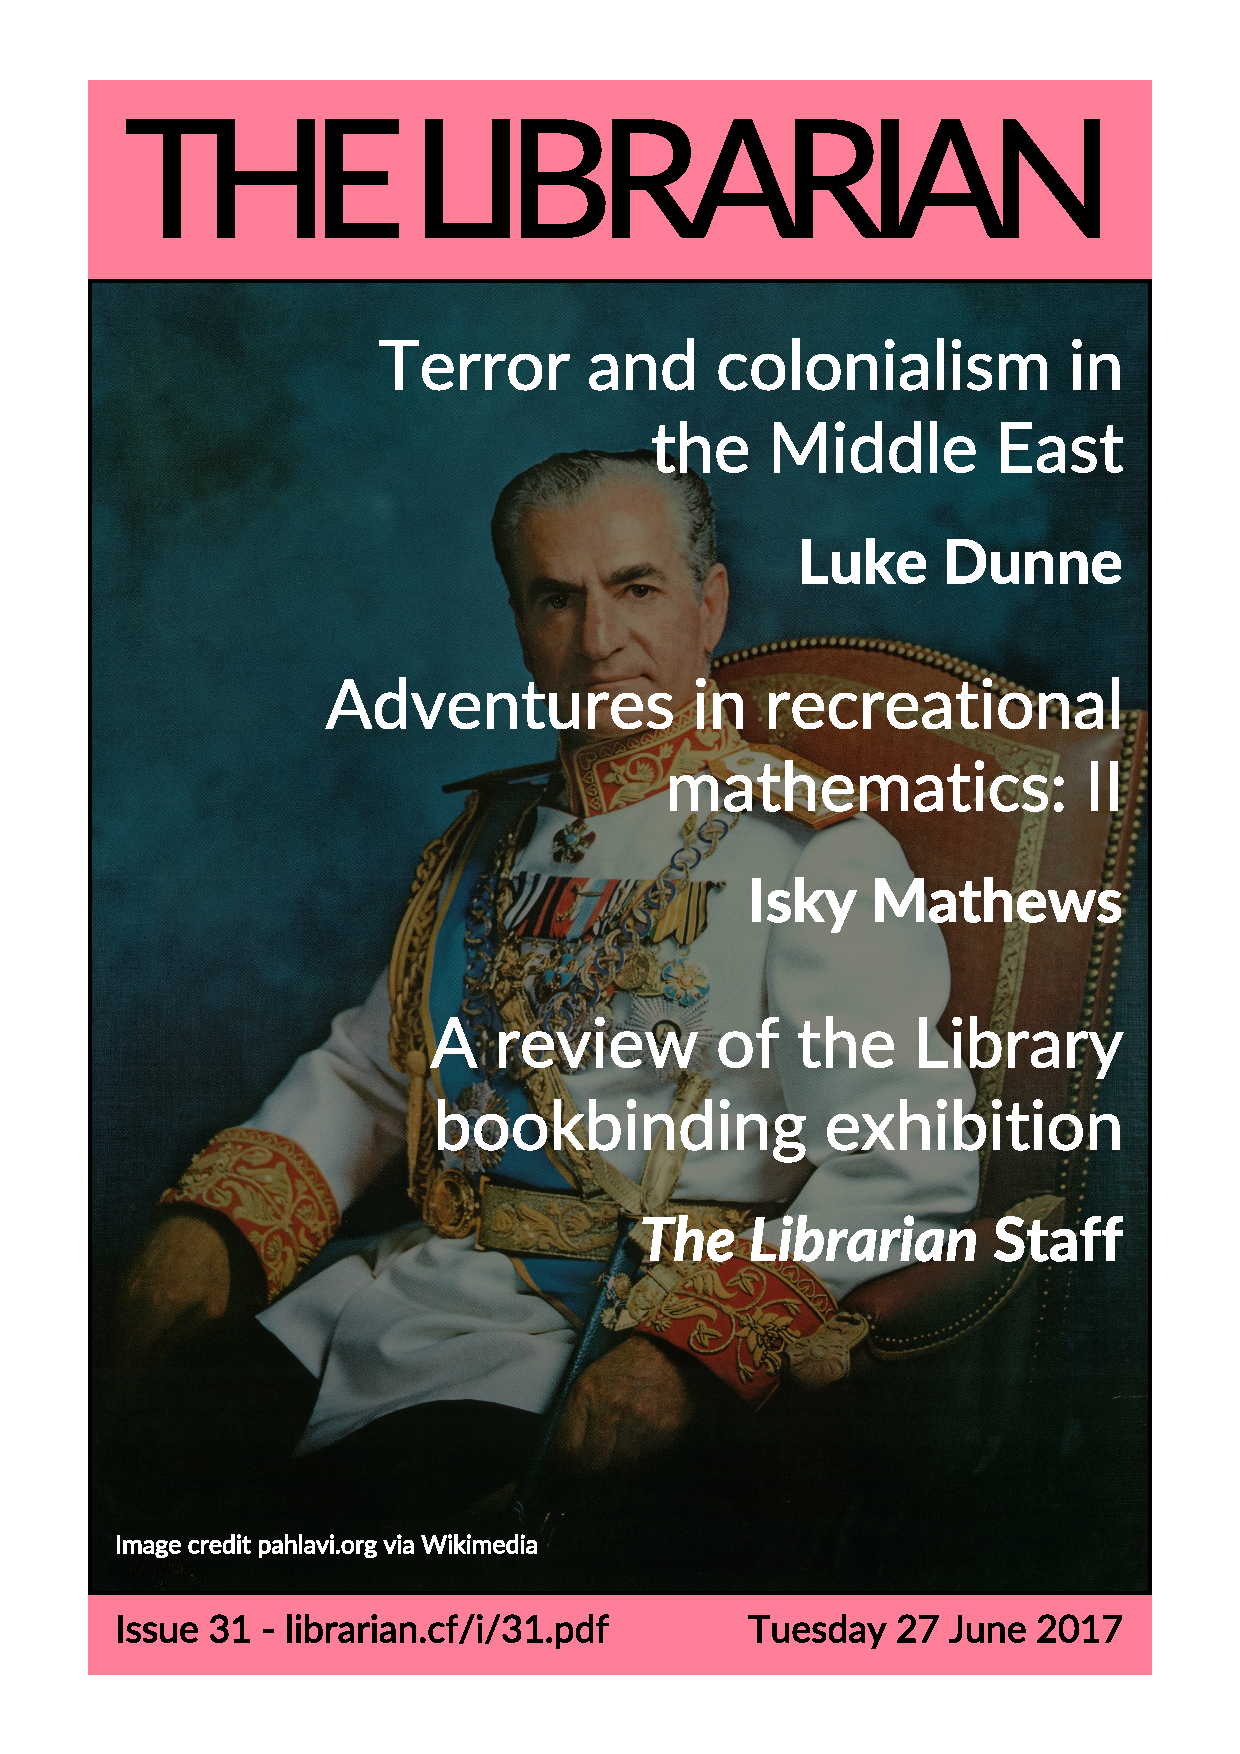
\includepdf[pages={1}]{cover.pdf}

\chapter{Library}

\begin{multicols}{2}

\section{Chair's welcome}

\begin{multicols}{2}
Welcome to our first edition of The Librarian this year, and we hope you enjoy it! The Librarian is The Library Committee’s monthly magazine, which you can find by the water dispenser in the Library, or by the entrance of the Library or up (most) houses (or wherever you got this copy from).

The Library is the one of the oldest parts of the school, and as libraries go, it’s a pretty impressive one. It is laced with history, being around in one form or another for hundreds of years. In the halls that we walk and work in, hundreds of years ago, librarians of the King kept the hugely historically important and significant artefacts and books that later formed made up British Library.

Even before the King’s Library, the very walls are steeped in history. If you walk to the back of the Library, the Greene Room and the Browne Room, or the vaulting ceilings of our 17th Century staircase tucked away in a corner showcase its restoration-era heritage. We share our library not just with each other, but with a rich architectural heritage and huge historical gravitas.

We are part of that heritage too, in a way. Nowadays, the Library is the hub of Westminster, and one with many different faces. For some, it’s a study resource, laden with information, key writings and vital texts. For others, it’s a quiet, productive space, with a studious atmosphere very conducive to hard work and vital revision. For many more, it’s a social space, where people can relax on a multitude of chairs and beanbags in what is a communal area for the entire school.

The Library is a part of every student’s life, no matter which subjects they take, which house they are in, which year they are in, and so it’s a huge honour to lead the Library Committee, a body where students can have their say in the running of the Library and where members can help with all the vital work the librarians and the Library do, from charity sales and helping students to sorting books.

It is hard to understate the role that the librarians do for us as pupils, and it weighs on me every time I enter the Library how difficult and vast a task it must be to look after the tens of thousands of books the school has, to organise and sort them into such a huge and useful tool for all students, and when one is in the Library Committee doing a fraction of their jobs, one really understands how thankful we should all be.

If you are new to the school, or if you haven’t really used the Library much before, use the opportunity, because it’s an incredible privilege to have such a historic, large, well-kept library and space, an opportunity many can only dream of having. For those who are new to the school, or reading this magazine for the first time, be sure to pick up your copy every month, and if you want to contribute, get in contact with Joshua Loo – and enjoy!

\subsection{An Invitation to the Library Committee}

The Library Committee is where pupils can get involved with the running of the Library. This means suggesting changes, talking with other pupils to find out what we could be doing better to make the Library more useful and accessible as a resource and more enjoyable a space for pupils not just of the upper years but throughout the school.

Members of the Library Committee also help as pupil librarians, setting aside some time in their busy weeks to work at the front desk, putting back books, helping pupils use the Library, and having what I find is a very enjoyable, quiet and productive space of time whilst making yourself very useful.

But the role of a pupil librarian, and the Library Committee, goes far deeper than that. With the great privilege of enjoying one of the finest and most historic libraries in Britain comes great responsibility to give back, and so at the Library Committee we help the Librarians in organising charity events and sales, the proceeds of which all go to charity.

The Library Committee also maintains \textit{The Librarian}, which is an exciting and forward thinking publication, taking contributions from both committee members and other members of the school community and weaving it into a magazine with very wide scope and high standards. If you have anything you’d like to contribute, email the editor at joshua.loo@westminster.org.uk.

If you are interested in joining the Library Committee, email me at jonny.heywood@westminster.org.uk, or just ask me in person, but remember, the role of a pupil librarian is one which requires a good deal of free time, a lot of patience, and obviously, a strong devotion to the Library. I hope to see some new faces soon!

Jonny Heywood, Chair

\subsection{Using the library}

The library may seem a daunting place at first. However, it is not actually very difficult to use. Books can be located at \url{https://oliver.westminster.org.uk} - use your Westminster login. If we do not have a book, you may suggest a book to the librarians by filling in a short form available in the library. Alternatively, speak to a librarian yourself. The librarians are always open to suggestions and very often accept them.

To find a book, first find its identifier on the Oliver search page. The first part of the identifier will be a number, eg. ``192''. In the front room of the library on the right of the doorframe to the left, there is a small sign which tells you which room the number will be in, and where the room is. The second part of the identifier is useful once you have found the room. It may simply be the first part of an author, eg. ``MIL'', or it may be another number. In any case, bookcases will have signage indicating which books are contained beneath them. They may indicate a range of numbers, or a range of letters.

The library has a number of other resources which are available on the library's Firefly page - \url{http://firefly.westminster.org.uk/library} or Firefly > Resources > Departments > Library. Online resources are contained on the eResources page. Particularly useful ones include JSTOR (good for sixth form especially), Naxos Music Library and the access to the archives and present articles of a nubmer of periodicals. The library itself receives many periodicals from across the world very frequently.

\end{multicols}

\section{Editor's note}

\begin{multicols}{2}

First, I should like to reiterate everything in the Chair's welcome. The Chair works very hard in his work with the Committee and the library as a whole.

I shall start with a few words on \textit{The Librarian}. We do not have any fixed subject. Rather, we publish anything submitted that we find intellectually stimulating. Articles must meet no requirements, save that they be intellectually stimulating and (negotiably) be less than 10,000 words. Importantly, \textit{The Librarian} \textit{does not represent the views of the Library Committee unless otherwise stated}.

\textit{The Librarian} also publishes \textit{Library News}, a one sheet publication containing library news, games, an agony aunt column and other such content.

This edition of \textit{The Librarian} has been redesigned, as our old readers may notice. This is largely due to inspiration from Felix O'Mahony, who supererogotarily submitted a design for the front page after submissions were sought for a favicon. The font size has also been increased from 10pt to 12pt, after a request by the Committee.

Adventures in Recreational Mathematics has taken an informatic turn, thanks to a stimulating submission from Benedict Randall Shaw. Isky Mathews wrote the past three adventures, and both form the team who publish it.

The cover photo is an image of Ataturk from Wikimedia Commons.

\textit{The Librarian} is now split into three primary sections:
\begin{enumerate}
	\item Dialectic,
	\item Review, and
	\item Sciences and Mathematics.
\end{enumerate}

\textit{The Librarian} is typeset in \LaTeX, with Scribus used to create the front page, in 12pt Lato and Computer Modern for mathematics.

The Editor would also like to remind readers that he accepts letters, agony aunt questions and game submissions.

To our old readers, welcome back! To our new readers, welcome!

\end{multicols}

\section{Addendum}

\begin{multicols}{2}
A number of editorial notices have been added to this edition after its initial publication for this web version. They relate to the librarians' clarification to the Editor that attacks on members of the school are not permissible. 

This edition is published for archival and historical purposes, and should not be construed as reflective of an ordinary \textit{Librarian} edition. 
\end{multicols}

\chapter{Dialectic}

\section{Headmasterly hand-wringing: avoidably fatuous and contentious}

\textbf{Joshua Loo}

\begin{multicols}{2}

The following note has been added for clarity.

\textbf{This article is not published in my capacity as the Editor of \textit{The Librarian}, nor does it represent the views of the library or the Library Committee. It is published in my personal capacity. The headmaster has discussed this article with me and raised no objection.
}

When the headmaster fatuously attacked protectionism as a false God, he
appeared to commit three sins. First, he exploited what ought to be a
neutral platform, ie. that of the headmaster in a school assembly, for
political ends. Second, there was no opportunity for reply, either in
the form of similarly vacuous hand-wringing or actual consideration.
Third, he failed to provide any analysis as to why his claims are true -
a rather dubious method by which one might follow a ``Gladstonian''
liberal tradition which presumably ostensibly embraces substantive
dialogue rather than empty rhetoric.

Yet as we explore how platforms in common institutions should be used,
we come up against a number of barriers in coherently defining a way to
exclude some but include others with a sufficiently nuanced and accurate
brush; not only this, it is difficult to generalise such rules so that
they apply from different ideological viewpoints.

Before that, we should note two recent pronouncements from the headmaster:
\begin{enumerate}
	\item The headmaster attacked Trump and protectionism in Latin prayers last term, and has repeatedly promoted his idea of Gladstonian liberalism.
	\item The headmaster claimed that the Armenian genocide was the first in the twentieth century.
\end{enumerate}

\subsubsection{Substance}\label{substance}

The point of speech which departs from that which has been
established\footnote{This is a somewhat confusing idea, which is
	difficult to define. Broadly speaking it includes what is either
	agreed with by everyone who is listening (eg. death is bad), is
	implicitly assented to even without actual agreement (eg. abbey
	service is compulsory) by some other action (eg. attending
	Westminster), is implied by anything which is already agreed upon (eg.
	that death is bad implies that Grenfell was a tragedy), or is the
	object of a broad scholarly consensus (eg. climate change is
	anthropogenic, Mathematics is true and Paris exists). An objection to
	the last statement was received in the writing process, so a
	modification to this is that this consensus can either be defined by
	the proportion of applicable persons who subscribe to a particular
	view, or in terms of the totality of the scholarly leanings of the
	community. The latter is to say that even if there is epistemic
	\textit{doubt} as to whether Paris exists, few scholars (unless
	attempting something weird semantically) will deny that Paris exists,
	and will merely attempt to induce doubt. If we total the overall
	leanings of a community where some are uncertain and others are more
	certain, all in one direction, we can say that there is some sort of
	consensus there too. This term will continue to be used throughout
	this essay. An addendum is that some of what is established is
	accepted for differing reasons; deontologists and utilitarians both
	agree that for all actions $x$, where $x$ only causes a
	death, $x$ is bad.
	
	Although these may seem intuitively true, they will each in turn be
	justified in the second section. Some of the latter subsets of
	``established'' truth are merely permissible because they form
	important subsets in turn of the first two.} is presumably to convince
us that there are more things which should be established; in turn, this
relies on the assumption that we should like to find truth. Given this,
reply is important. An initial argument is not necessarily correct;
corrections are important. Even if the original thesis of an argument
turns out to be correct, the process of rebuttal strengthens arguments -
knowing the same truth for better reasons is itself desirable. Finally,
reply, and further replies in turn, increase the perception that truth
has been found. When a good process for finding the truth has been
found, ie. argument, it is important that other people recognise its
validity, the more to transmit truth.

Protectionism's lack of efficacy has not been established in three ways.
First, it is unclear which moral system is best used to determine what
is good or bad. A ``utilitarianism of money'', which blindly seeks the
greatest gross global product, would differ in its recommendations to
preference utilitarianism, Rawlsian justice as fairness in its original
moral formulation, or rights theory. Second, even practising a
Li-style\footnote{Li, S. (2017) ``Ethics and Market Design'', accessed
	via shengwu.li} ``informed neutrality between reasonable ethical
positions'', it is not clear whether protectionism ``works'' - Ha-Joon
Chang writes that protectionism in some forms was crucial to
industrialisation in a number of countries\footnote{Chang, Ha-Joon
	(2002) \textit{Kicking Away the Ladder: Development Strategy in
		Historical Perspective.}}, in a tradition of correlated protectionism
and development stretching back at least to high American tariffs in the
19\textsuperscript{th} and early 20\textsuperscript{th} century, South
Korea's rapid industrialisation and a number of other examples; this
industrialisation and the concomitant reduction of human misery are
presumably good things in all reasonable ethical positions. Third, at no
point was it established as a founding truth for the school, nor was it
acknowledged or assented to. We may, for example, implicitly agree not
to be violent to each other, with all the constraints on the full
implementation of certain ideologies this entails, in going to school;
we do not agree to the headmaster's Gladstonian liberalism in its full
muscular ``glory''. Hence in this sense, what the headmaster does not
fall into the set of established ideas which are broadly acceptable.

What sort of principles should be applied to those who wish to depart
from what has been established, in terms of their presentation?

First, and perhaps most importantly, they must act so as to maximise
truth. There was little chance of anyone shouting in reply ``no it
isn't'' to the headmaster without sanction; this is obviously a
relatively trivial barrier to remove. Replies must be available, and
listened to by everyone who listens to the original; if attendance is
compulsory, attendance to the reply must also be compulsory, so that
reply actually works. They must also be given sufficient time, and due
notice. Additionally, any form of sanction oughtn't to exist. They may
inevitably exist unless the headmaster is, for example, stripped of all
power within the school, but need not unnecessarily exist. It mustn't
necessarily be the case that everyone is afforded the opportunity to
speak. It is however, desirable that at the very least an opposing
viewpoint is heard.

Second, and relatedly, these views mustn't be presented as established.
A headmaster appears to hold the full force of the coercive and
administrative apparatus of the school. It must be expressly stated that
whatever he says is not the view of the school if it is not established
as such. This separation must be made clear so as to enable the full
implementation of the first principle\footnote{The theme of the effect
	of authority is continued later, in ``Neutrality: a desideratum?''.}.
This was not done.

Third, these views must be important. There is limited time and limited
space for discussion. Importance can be defined in a moral sense - the
imparting of important moral truths, ie. what \textit{ought}, can be said
to be important, and we can measure importance in this way. Truths as to
what \textit{is} are also important\footnote{This is in reference to the
	is/ought distinction; see Hume's \textit{A Treatise of Human Nature},
	Book III, Part I, Section I, p. 469. Hume notes that we cannot
	determine what ``ought'' to be the case, ie. moral truth, without at
	least one other such truth; without any, we cannot say that anything
	is bad. An example may clarify: ``$x$'s sole consequence is a
	death'' does not imply that ``$x$ is bad'' unless we also accept
	the moral premise that ``we oughtn't to murder'', or ``death is bad''.
	``Is'' statements may imply ``ought'' statements in conjunction with
	other ``ought'' statements. Though this is the case, following Li's
	model of ``informed neutrality between reasonable ethical positions'',
	we can take some ought-conditions to be given (eg. death is bad), and
	so consider things which affect lots of people, and therefore may
	interact with ought-conditions, to be important as well, though they
	only describe what is.}, if they are important based on two kinds of
ought. The first is when an ought is already established. The second is
when the case that something ought to be the case is made in the same
way, as described before.

The lack of desirability of the third sin is uncontroversial. Those who
decry protectionism likely seek a better justification and presentation
of this view than what occurred in Latin prayers. Those who support it
would simply note the falsity of his claim. It is not particularly
controversial to seek an amelioration in standards of discourse, though
the headmaster is not alone in dialectic moronisation and is perhaps
better than certain others in his ability to orally extemporise a series
of grammatical English sentences, each with a main verb, unlike some of
the present ``friends'' of one (now part-time) occupant of Chequers.

Hence we add another two principles. Fourth and relatedly, views must be
rigourous and have a moderate chance of success, even if they do not
fully convince. This is partly related to the third principle, ie. that
of prioritisation, but it is also because poorly justified views are
more likely to be incorrect than rigourously justified views, insofar as
ordinarily that true views are more easily justified.

Fifth, nothing in these principles fails to apply to the assumptions,
anecdotes, quotes and any other topics during all compulsorily attended
discourse. An inadvertent denial of the Herero and Nama genocide in
German-ruled Namibia by terming the Armenian genocide ``first'' in the
twentieth century would be unacceptable even were it not to be a main
message.

\subsection{Neutrality: a
	desideratum?}\label{neutrality-a-desideratum}

The solution to the first sin, whether in Liberty University's
compulsion of students to listen to Ted Cruz\footnote{It appears that
	this also occurs with other speakers, eg. Bernie Sanders, as part of a
	weekly assembly. Liberty University is questionable in a number of
	ways but the imbalance in speakers appears to be caused by progressive
	speakers' refusal to accept invitations to speak.} or Westminster's to
the Headmaster appears to be neutrality. Compulsory school meetings
ought to simply be about school - fire drills, timetabling, achievements
and other educational minutiae. This has a certain appeal - it seems to
be functional (who gains from vacuous hand-wringing?), fair, and clear.

\subsubsection{Is compulsorily attended dialectic discourse
	helpful?}\label{is-compulsorily-attended-dialectic-discourse-helpful}

Compulsory discourse which is overtly dialectic causes three harms.

First, it alienates those who disagree with the message it spreads.
Although this may not seem like a harm in all circumstances, eg. if it
alienates racists, the neutrality of institutions is itself a good in
that it enables different otherwise mutually incompatible sections of
society to cooperate. Consider, for example, rubbish collection: if
rubbish collection is politicised (eg. if all rubbish bins were to be
painted with anti-racist slogans), it is possible that those who
disagree (even if they are wrong\footnote{The effect described here is
	plausibly more likely to occur when the group who disagree with a
	politicisation attempt have poorly justified views; poorly justified
	views are more likely to be grounded in some sort of blind faith,
	whether religiously or socially motivated, and so they are plausibly
	held with much more faith and strength than views which are based on
	other views and are somewhat instrumental. Contrast two opponents of
	euthanasia, the first of whom believes that it is biblically
	forbidden, the second likely to cause people to be forced into
	coercion. The former will be very hard to convince - biblical
	teachings are hard to rebut - compared to the latter, who may be
	convinced that this coercion is less important than the coercion
	experienced by those forced to live, or that it is very unlikely.})
will stop cooperating with rubbish collection. This is bad because
rubbish collection is environmentally important.

Second, it unfairly advantages certain points of view. Arguments cannot
be agreed with if they aren't heard. Where there is compulsory
discourse, it is often delivered by an authority figure - a headmaster
or a graduation speaker, to take a few examples. Listeners may view such
discourse with undeserved respect. This is not to say that these figures
cannot be correct, but rather that they are less likely to be correct
than the people whom would be trusted by the force of their argument,
unbuttressed by the perceived stature which many of these authority
figures possess.

Third, it alienates those who do not wish to listen to dialectic
reasoning. Compulsory attendance already is sufficiently coercive to
cause resentment. This resentment is compounded by the addition of
seemingly unneeded dialectic speech. Why must more of their time be
wasted? They are not listening - they are worse than idling, for they
who must listen unwillingly to headmasterly pronouncements on
Gladstonian liberalism are not enjoying themselves. Even if a lack of
interest is to be decried, one's aim oughtn't to be to maximise the
misery of the uninterested but to increase their interest. This feeling
of resentment is entirely unnecessary; it reduces the likelihood that
individuals will naturally gravitate towards interest, which will
produce a superior organic and sustainable interest.

This harm must be weighed against the benefit to, to continue this
example, the people who feel supported by anti-racist slogans. The
benefit is not only not particularly large, but also is not uniquely
achieved by such an action. There are many other ways to promote
anti-racism and make oppressed racial minorities feel happy. Where there
are other avenues open which directly concern a matter\footnote{Consider
	harsher penalties for racial abuse, a privately funded publicity
	campaign or an outreach programme.}, one oughtn't to use institutions
whose specific purpose would be negatively impacted.

If there are no such avenues, such action ought to be permissible only
if it meets two conditions.

First, the harm to, for example, rubbish collection, must be minimised,
in attempting to use the least destructive means possible, using the
previous set of avenues to the maximum extent possible and so on. This
ought to be fairly obvious.

Second, benefit must outweigh systemic and immediate harms to, to
continue the example, rubbish collection. We must consider all the extra
rubbish which will be incorrectly sorted, littered or thrown into rivers
etc.; we must consider the harm to cooperation with other council
services as well. Insofar as this is very difficult to quantify and
predict, the second condition must be modified such that, out of an
abundance of caution, the smallest reasonably likely set of benefits
must be larger than the greatest reasonably likely set of harms to
accrue. This is because systemic harm is very difficult to rectify. At
worst, it looks like the tribal epistemics that are described by David
Roberts\footnote{\textit{vide}
	https://www.vox.com/policy-and-politics/2017/3/22/14762030/donald-trump-tribal-epistemology},
where institutions are abandoned wholesale to the point that having
common institutions at all which help us to find the truth, like
universities (whose research helps to improve society by telling us
about problems and how to fix them), neutral government institutions
(who have a similar function - not to deliberate about what ought to be
the case but to implement ought-conditions given to them by governments
and tell the public about what \textit{is} so that they can figure out
what ought to be) and, just as important if not more so, a free press,
becomes increasingly unworkable due to a lack of public buy-in. Notably,
there are few easy solutions once this road is gone down. It is unclear
how, if at all, the mainstream press is to regain the trust of those who
are convinced that it is now in the pay of globalist conspirators. All
neutral institutions are potentially subject to the same level of
abandonment, which greatly diminishes their utility. To err on the side
of caution, therefore, is only a logical conclusion of this\footnote{See
	other discussion related to the precautionary principle; the
	precautionary principle is a similar principle, where certain threats,
	although distant and somewhat unquantifiable, can be justified to
	restrict actions, due to their large magnitude. It applies to health
	and the environment, instead of a risk of abandonment of institutions.}.

If the headmaster insists on using his platform for the propagation of
dialectic material in the manner he has done so, it's clear that he
risks incurring systemic harm of the same sort.

First, those who agree with his statements may benefit. However, they
will not particularly benefit - a headmaster's consolation is not
insubstantial but it is not clear that it is particularly large.
Moreover they are capable of reading things they agree with in other
places, at other times, by authors more reputable (since their
livelihoods may be based on writing about the economics which the
headmaster of a school is not \textit{ex oficio} concerned with). Hence we
can largely discount this benefit.

Second, those who disagree with his statements are less likely to
identify with the headmaster, and, by extension, the school. This is
problematic in two ways. First, it undermines respect for the
institutions of the school - they are viewed not as neutral arbiters but
as part of ``the other side'' - in this case, the ``liberal'' side. This
is problematic in the same way as the rubbish collection example
describes. Cooperation with school authorities is important in a number
of respects - it helps to maintain safety, it qualitatively ameliorates
learning, it results in smoother administration and reduces costs, and
so on. The headmaster sacrifices this not only at his peril but at the
school's peril, for systemic harms like this will last after his
departure. Second, it reduces the openness with which views are
expressed. This is a somewhat independent harm. Views which aren't heard
are less likely to be held because probabilistically they are unlikely
to be independently be developed; their lack of audience is orthogonal
to their truth. This violates the second principle established in the
first section of this essay.

Third, this harm is compounded by an innate adolescent contrarianism,
and unjustifiably permits those who go against liberal orthodoxy to
claim the intellectual high ground. That adolescent contrarianism is
beyond the scope of this essay; assuming that it exists, heavy and
burdensome imposition appears to be unhelpful in changing attitudes for
the better. Moreover the headmaster's insistent use of rhetoric, as
opposed to analytic argument grounded in an instrumental rationality
whose values can broadly be accepted by those whom he ought to seek to
convince\footnote{If he is not attempting to convince, he is merely
	virtue-signalling, which is clearly not worth our time.} allows his
lack of analysis to be ridiculed as indicative of poor reasoning on the
part of all those who seek to promote, for example, free trade, or
socially liberal values.

\subsubsection{Is neutrality possible?}\label{is-neutrality-possible}

In short, not particularly, but we have a workaround.

All statements either contain an implicit or explicit assumption as to
what is important or admit their unimportance. Consider statements about
fire alarms. This assumes that fire alarms are impossible (because fire
alarms help to prevent death which is bad, and that death is bad is
important).

Implicit assumptions as to what is important do not necessarily make a
statement unimportant. We take lots of things as implicit;
mathematicians take some very basic mathematics as implicit, eg. the law
of identity, but we do not criticise them for that (much).

Given this, ``neutral statements'' also contain dialectic statements
themselves as to what is important. These are in the same class as
``ought'' statements - ``$x$ is important'' can broadly be mapped
to ``one ought to prioritise $x$'', and ``$x$ is more
important than $y$'' can be mapped to ``one ought to prioritise
$x$ over $y$''.

Hence by default the principles stated at the beginning of this essay
for non-established claims apply.

However, there are four exceptions to this rule.

First, if everyone in a community agrees on a specific ``is'' or
``ought'' statement (eg. ``education is utile'', ``students will take
GCSE examinations'' and ``water will be provided to students''),
reminders, clarifications and so on are all permissible, without
specific reference or resort in line with the principles enumerated
earlier. This is because the implementation of a pre-agreed ``is'' or
``ought'' oughtn't to require agreement again.

Second, we take assent without belief to constitute agreement.
Attendance of this school is voluntary; the vast number of schools which
exist and the lack of coercion on the part of the school mean that we
can take the school to be engaged in an ordinary contractual interaction
with parents and schoolchildren\footnote{Contrast, for example, the
	state, which may not do certain things due to its position as already
	here. Note further the inapplicability of a potential argument against
	claims reliant on choice: in an example where there are ten prisoners
	in a cell and one key, the ten prisoners are not said to be free even
	though they may be each individually able to escape, but the situation
	is disanalogous - there is no necessity that one joins the school, and
	there is sufficient liquidity experienced, at least by almost all
	those who go to this school, to say that this argument would not apply
	anyway because everyone within the school is able to choose somewhere
	else.}. Hence that the ethos of the school involves the protection of
the wellbeing of all students to some equal degree in outcome in all
students means, for example, that even if one were to think
otherwise\footnote{Consider certain homophobic religions.} and disagree
the school may still act based on it, and so pronouncements in assembly,
for example, about such matters are also permissible.

Third, what is trivially derived from anything in the former two also
ought to be included as an exception. This is because parents accept
that there is a degree of uncertainty as to the outcomes of a school's
axiology, as it were. They accept the school's axiological premises,
instead of particular outcomes.

Fourth, in a school environment, certain things are necessarily accepted
as part of the former three exceptions. Schools accept mainstream
academic thought in that they teach it. This is accepted by attendance.
It is therefore permissible to, for example, take as established that
there exists anthropogenic climate change, even if parents have not
accepted this, by the second principle\footnote{See footnote 1 for
	further clarification of the idea of a consensus.}.

The former three exceptions can be applied to other institutions too. A
rubbish collection company may promote respecting recycling sorting
procedures without falling foul of the principles established before.

\subsection{Conclusion}\label{conclusion}

First, we establish five principles which apply to the strength and
presentation of dialectic compulsorily attended events. We also
establish that the headmaster failed to meet four of the five principles
at various times, and what he did failed to qualify for an opt-out as
``established''. Second, we show that overtly dialectic compulsorily
attended events cause three harms, the last of which is systemic. Given
this systemic nature, two principles apply: first, that all alternatives
should be maximally used, and second that if this is insufficient to
avoid using publicly shared institutions, we should use extra caution,
and so the smallest reasonably likely set of benefits should exceed the
largest reasonably likely set of harms. Third and finally, we show that
there are some opt-outs based on what is pre-agreed.

There is a broader problem here, which has not been identified so far.
It relates not so much to the principles espoused here as the sense of
entitlement which is felt by those who exploit common institutions in
this way. It is shared by the proms conductor who felt that the beauty
of Beethoven's Ninth was insufficient as a plea for our common humanity
and so his vastly inferior words had to compensate and those who thought
his words appropriate and utile. Its manifestation is in the growing
departure from any pretense of neutrality on the part of some of the
institutions which need it most - schools and universities, the press
and other common institutions. It is a complete ignoring of systemic
considerations - a sand castle of an institution is one which is
brittle, and when cracks start to appear, that a little water will
appear to fix is no consolation, for the sand castle is doomed thence to
fall.

\end{multicols}

\chapter{Review}

\section{Crooke's \textit{Resistance}}
\textbf{Joshua Loo}

\begin{multicols}{2}

Discourse about Islam often blithely assumes Islamic inferiority,
whether in overtly advocating its suppression or appeasement.
\textit{Resistance}'s dual account of Islamic intellectual history from
the breaking up of the old Ottoman order to the modern structure of
Hamas and Hezbollah and the religious roots of the instrumental
rationality of Western orthodoxy is no less relevant today than they
were at their publication in 2009.

Crooke's account of the imposition of westernisation is not particularly
novel, but it is written well enough, and is quite passable. His
critique of Western instrumental rationality, though somewhat incomplete
and lacking in philosophical depth, is far from inaccessible, and
contains a number of useful insights. Again, this account is not
completely novel, but it is still adequate.

The granting of equal status to Islamist ideology enables an interesting
and perhaps novel comparison with the Western intellectual canon. The
book shines when it questions the distinction often drawn between
Western intervention and Islamist jihad. Its praise of Islamism as an
open ideology, and the distinction drawn in action and philosophy
between the eschatology of Al Qaida and the ``emancipatory resistance''
of Hamas and Hezbollah is another highlight. \textit{Resistance} contrasts
this with the religious roots of Western just war theory.

The book is moderately well written. It has a relatively wide frame of
reference, as would be expected of a book with its thesis. Occasionally
it is a little difficult to follow due to unintuitive sentence
structure, but that itself is no major crime. Although accessibly
written, it has not obviously reduced the complexity of the ideas that
it presents.

However, Crooke ignores a number of issues which would complete and
round his account. Though Western ideology may have its flaws as he
posits, he ignores a number of problematic views and actions in these
groups. Consider that Hamas's 1988 charter, which is still in force,
mentions a ``struggle against the Jews'' and approvingly quotes:

\begin{quote}
	"The Day of Judgement will not come about until Moslems fight the Jews
	(killing the Jews), when the Jew will hide behind stones and trees. The
	stones and trees will say O Moslems, O Abdulla, there is a Jew behind
	me, come and kill him. Only the Gharkad tree, (evidently a certain kind
	of tree) would not do that because it is one of the trees of the
	Jews."\footnote{http://avalon.law.yale.edu/20th\_century/hamas.asp}
\end{quote}

Any attempt to legitimise such movements must also account for this.

The Middle East Media Research Institute, an organisation which has been
accused of deliberate mistranslation or misleading translation in the
past, but whose translations are rarely completely incorrect, reported
that the Secretary-General of Hezbollah declared that homosexual
relationships were ``contrary to logic, human nature and the human
mind''\footnote{https://www.memri.org/tv/hizbullah-sec-gen-nasrallah-warns-against-legalization-gay-marriage-lebanon-defends-early/transcript}.

These issues may not be as large has is otherwise suggested, but they
still ought to have been addressed.

Nevertheless, it is still well worth reading.

\textit{Resistance: the essence of the Islamist revolution} is available
in the library, or will be when the Editor has returned it.

\end{multicols}

\chapter{Sciences and Mathematics}

\section{Adventures in (informatically simulated) recreational mathematics: An introduction to big-O notation, and these plural heresies with which to conduct multiplication with increasingly full vigour}

\textbf{Benedict Randall Shaw}

\begin{multicols}{2}

DISCLAIMER: this edition of ARM contains neither traditional maths nor any pretty pictures; rather, we are stepping out into the related field of computer science, and are stuck with graphs. We apologise for any inconvenience caused.

\subsection{Big-O Notation}

In computer science, one seeks to write efficient algorithms, so as not to waste valuable processing time. However, as counterintuitive as it sounds, what we care about most is not how well a program performs on a given value, but rather how well it scales to more complex situations.\\

\end{multicols}

\clearpage

\parbox{0.333333333\textwidth}{\centering
	\includegraphics[width=0.33333333333\textwidth]{smallgraph}
	Figure 1}
\parbox{0.333333333\textwidth}{\centering
	\includegraphics[width=0.33333333333\textwidth]{mediumgraph}
	Figure 2}
\parbox{0.333333333\textwidth}{\centering
	\includegraphics[width=0.33333333333\textwidth]{largegraph}
	Figure 3}\\

\begin{multicols}{2}

Consider three programs which sort a list of length \(n\), which we'll call the red, blue, and green programs. We now graph the worst-case (longest) period of time required for each of these programs against the lengths of list, shown at different scales in Figures 1, 2, and 3. From Figure 1, it would seem that the green program is the quickest; however, for most values it turns out to be by far the worst. We don't usually care about comparing the time taken to sort short lists, as this can be done very quickly either way, and the differences in time taken aren't actually that large. What we care about are cases where the list is long, as shown on the far right of Figure 3, as the slowest programs can take many times to longer to run than the fastest. In fact, in many such problems, even algorithms which both look at the small scale to be similar (e.g. the blue and green programs) grow to be have very different performances eventually. Computer scientists describe the rate of growth of running times using \textit{big-O notation}.

We say that \(f(n)=O(g(n))\), where \(f\) and \(g\) are functions on the real numbers, if there exist positive real numbers \(M\) and \(y\) such that for all values of \(n \geq{} y\), \(|f(n)|\leq{}|Mg(n)|\). At face value, it may seem that by making \(M\) very large, any program must take less than \(Mg(n)\) units of time to run. This is not the case, as can be illustrated with \(f(n)=n^2\) and \(g(n)=n\); for any value of \(M\), for all values of \(n>M\), \(f(n)=n^2>Mn=Mg(n)\) as \(n>M\), so \(f(n)>Mg(n)\) eventually for all values of \(M\). What we really mean in a nutshell by \(f(n)=O(g(n))\) is that \(f(n)\) doesn't grow more quickly than \(g(n)\)\footnote{This phrasing is a slight oversimplification, but helpful to consider in order to understand the concept.}. There are a variety of other pieces of big-O notation. For example, we say \(f(n)=\Omega(g(n))\) if there exist positive real numbers \(N\) and \(z\) such that for all values of \(n \geq{} z\), \(|f(n)|\geq{}|Ng(n)|\); this essentially means that \(f(n)\) doesn't grow less quickly than \(g(n)\)\footnotemark[\value{footnote}]. We also say that \(f(n)=\Theta(g(n))\) if \(f(n)=O(g(n))\) and \(f(n)=\Omega(g(n))\) (that is to say, if \(f(n)\) grows roughly as quickly as \(g(n)\)\footnotemark[\value{footnote}]).

Interestingly, if a function \(f(n)=g(n)+h(n)\), and \(g(n)\) grows at least as quickly as \(h(n)\), and \(g(n)=O(d(n))\) for some function \(d\), then as past a certain point \(g(n)\geq{}h(n)\), and past said point \(f(n)\leq{}2g(n)\leq2Md(n)\), so \(f(n)=O(d(n))\) too (as \(f(n)\leq{}2Md(n)\) and \(2M\) is a constant real number). What this really means is that a function grows as quickly as its fastest growing term; for example, if \(f(n)=2x^3 + 5n^2 + 2\log()n + 11\), then \(f(n)=O(x^3)\) as \(2x^3\) grows more quickly than the other terms. For this, it is helpful to have some idea about which functions grow more quickly than others; a chart of such functions is given at the end of this section.

In computer science, we care predominantly about the worst-case running time; it (usually) causes no problems if a program runs quickly, but a program taking ages to run is to be avoided if the program is to be usable. We therefore tend to prioritise \(O\) over \(\Omega\) and \(\Theta\). We say a program has \textit{time complexity} of \(O(g(n))\) (or sometimes we just say that it is \(O(g(n))\)) if its worst case running time in arbitrary time units is \(O(g(n))\); for example, the red program in Figures 1--3 is linear and so has time complexity \(O(n)\). (It is also technically \(O(n^2)\), as \(n^2\) grows faster than a linear function, but this is unhelpful, so the time complexity uses the slowest growing function we can possibly place inside the brackets of \(O()\).) We have names for some time complexities; for example, we say the red program has linear time complexity, for obvious reasons. Below is a chart of common time complexities and their names, ordered from slowest to fastest growing.

\end{multicols}

\begin{center}
	\begin{tabular}{c|c}
		\(O(1)\)&constant\\\hline
		\(O(\log*n))\)&log-star\footnotemark\\\hline
		\(O(\log(\log{}n))\)&double logarithmic\\\hline
		\(O(\log{}n)\)&logarithmic\\\hline
		\(O(n^c)\) where \(0<c<1\) is a constant&fractional power\\\hline
		\(O(n)\)&linear\\\hline
		\(O(n\log{}n)\)&linearithmic\\\hline
		\(O(n^c)\) where \(1<c<2\) is a constant&polynomial\\\hline
		\(O(n^2)\)&quadratic (also polynomial)\\\hline
		\(O(n^c)\) where \(2<c<3\) is a constant&polynomial\\\hline
		\(O(n^3)\)&cubic (also polynomial)\\\hline
		\(O(n^c)\) where \(3<c\) is a constant&polynomial\\\hline
		\(O(c^n)\) where \(1<c\) is a constant&exponential\\\hline
		\(O(n!)\)&factorial
	\end{tabular}
\end{center}
\footnotetext{\(\log*n\) is the number of times the logarithm function must be iteratively applied to \(n\) before \(n\leq{}1\).}

\begin{multicols}{2}
	
\subsection{Long multiplication}
It is necessary for a computer to be able to carry out arithmetic operations as quickly as possible, as these are the building blocks of most programs. We can add two \(n\)-bit\footnote{binary digit} numbers (those less than \(2^n\)) with \(O(n)\) time complexity on a sequential circuit through the usual method that one is taught in school; one simply goes through the two numbers bit by bit, starting with the least significant, and adds them, carrying over into the next column if one needs to. One must only ever add a maximum of three bits (two from the numbers and one from carrying) each time, each individual bit addition has constant time complexity. Because one goes through \(n\) such sets of bits, addition has \(O(n)\) time complexity.

Multiplication is trickier. However, in the same way that we find it very easy to multiply by powers of 10 by adding zeroes, modern computers are able to multiply by powers of two with \(O(1)\) time complexity (using a circuit called a barrel shifter which will not be explained here). This is called a bit shift, and is very helpful. It means that the long multiplication algorithm, which probably we have all used at some point or other, can be done fairly quickly on a computer. For two \(n\)-bit numbers, long multiplication gives us an intermediate term for each \say{1} bit of the first of the numbers to be multiplied. In the worst case scenario, there are \(n\) of these terms, and as each is produced in constant time from bit shifts, the production of these has \(O(n)\) time complexity.

As they are all the product of an \(n\)-bit number and a power of two that fits in \(n\)-bits, the terms fit in \(2n\) bits. Thus we are adding \(n\) \(2n\)-bit numbers, so we must perform \(n-1\) addition operations. As addition is \(O(n)\), this means that the summation of the intermediate terms has \((n-1)\times{}O(2n)=O(2n^2-2n)=O(n^2)\) time complexity. The production of the terms is \(O(n)\), so the time complexity of long multiplication is \(O(n)+O(n^2)=O(n^2)\). This is pretty bad. If we wanted to multiply two ten-million-digit numbers (33 million bits), and we were able to perform a billion single-bit additions a second, this algorithm would take nearly a fortnight.

\subsection{Karatsuba's algorithm}

It was conjectured by Andrey Kolmogorov, a notable Soviet mathematician, that the quadratic time complexity of long multiplication could not be improved upon. In 1960, he held a seminar at which he mentioned this, among other computational complexity problems. A week later, Anatoly Karatsuba, a 23-year-old student, found this algorithm, which runs with \(O(n^{log_{2}3})\approx{}O(n^{1.585})\) time complexity.

It belongs to a class of algorithms known as \say{divide and conquer} algorithms. These work by splitting problems into smaller instances of the same type of problem, until they can be solved easily, and then recombining the solutions to solve the initial problem.

Consider multiplying two \(n\)-bit integers, \(x\) and \(y\). Let \(m\) be \(\left\lceil\frac{n}{2}\right\rceil\). Then by splitting \(x\) and \(y\) down the middle, we can obtain \(x_1,x_0,y_1,y_0<2^m\) such that \[2^{m}x_1+x_0=x\]\[2^{m}y_1+y_0=y\]
Then it follows that \[xy=2^{2m}x_1y_1+2^m(x_1y_0+x_0y_1)+x_0y_0\]
There are 4 multiplications to be performed here, and one method of multiplication has you do them all individually; then one does those multiplications by the same technique, and so on until the multiplications are all single-bit, upon which you do them by the usual method. Suppose it takes \(T(n)\) basic operations (single-bit additions and multiplications) to multiply two \(n\)-bit numbers by this method; then this method gives \(T(n)=4T(\left\lceil{}\frac{n}{2}\right\rceil{})+6n\), as we have to add 4 \(2n\)-bit numbers, which require 3 additions (so require \(6n\) basic operations in total).

This is called a recurrence relation, and can be solved by through a variety of means. For the sake of brevity, we shall use the master theorem, which tells us that, where \(T(n)=aT(\frac{n}{b})+f(n)\), and \(c_{crit}=\log_ba\) (the \textit{critical exponent}): when \(f(n)=O(n^c\) for some \(c<c_{crit}\) (i.e. the work to split and recombine a problem is far less than that of the subproblems), \(T(n)=\Theta(n^{c_{crit}})\); when \(f(n)=\Theta(n^{c_{crit}}log^kn)\) for some \(k\geq0\) (i.e. the work to split and recombine a problem is comparable to that of the subproblems), \(T(n)=\Theta(n^{c_{crit}}log^{k+1}n)\); and when \(f(n)=\Omega(n^c)\) for some \(c>c_{crit}\) (i.e. the work to split and recombine a problem is far greater than that of the subproblems), \(T(n)=\Theta(f(n))\).

In the case of the algorithm we are currently considering, \(T(n)=4T(\frac{n}{2})+6n\) (we have dropped the ceiling signs, as they make a tiny change in the grand scheme of things to \(\frac{n}{2}\) which does not affect the time taken significantly). Thus \(c_{crit}=\log_{2}4=2\) and \(f(n)=6n=O(n^1)\) so \(c=1<c_{crit}\). The master theorem then tells us that \(T(n)=\Theta(n^2)\), which is no better than long multiplication.

What Karatsuba hit upon was that \[xy=2^{2m}x_1y_1+2^m(x_1y_0+x_0y_1)+x_0y_0\] could be calculated with only 3 subproblems. We calculate \(z_2=x_1y_1\) and \(z_0=x_0y_0\). Then we calculate \(z_1=(x_1+x_0)(y_1+y_0)-z_2-z_0\), which is equal to \(x_1y_0+x_0y_1\). Thus we have only made three multiplications, and a couple of additions and subtractions, both of which have linear time complexity. Thus Karatsuba's algorithm gives us \(T(n)=3T(n/2)+f(n)\), where \(f(n)=O(n)\). By the master theorem, \(c_{crit}=\log_{2}3\), so as \(f(n)=O(n^1)\), \(c<c_{crit}\), and \(T(n)=\Theta(n^{\log_{2}3})\approx{}\Theta(n^{1.585})\).

This means that in our previous example of two ten-million-digit numbers, we would be done in a couple of hours. This is a marked improvement, but we can still do better.

\subsection{Toom-Cook}
In 1963, Andrei Toom described a generalisation of the Karatsuba algorithm, which Stephen Cook improved as his PhD in 1966. It uses the technique of splitting numbers up (as in Karatsuba) and treating them as polynomials, which is also used in the Sch\"onhage-Strassen algorithm, which is faster still.

Long multiplication is Toom-1, and has time complexity \(=O(n^2)\). The Karatsuba algorithm is Toom-2, and has time complexity \(\approx{}O(n^1.585)\). Toom-3 has time complexity \(\approx{}O(n^1.465)\). In general, Toom-\(k\) has time complexity \(\Theta(c(k)n^{log(2k-1)/log(k)})\), where \(c(k)\) is the time spent on addition and multiplication by small constants. Unfortunately, the function \(c(k)\) grows very quickly. Through use of a variety of values of \(k\), Donald Knuth has made a Toom-Cook implementation that runs in \(\Theta(n2^{\sqrt{2\log{}n}}\log{}n)\) Due to overhead, Toom-Cook is slower than long multiplication for small numbers. We shall consider Toom-3 as an example; however, we shall give the general algorithm of Toom-\(k\) for any value of \(k\).

Given \(n\)-digit numbers \(x\) and \(y\) (we'll use \(31415926\) and \(2718281\)), we start by splitting each into \(k\) digits in some base \(B=b^i\) for some integer \(i\), where we have the numbers in base \(b\).
Let these \(k\) digits of \(x\) be the coefficients of a polynomial \(P\), and those of \(y\) be coefficients of a polynomial \(Q\). These polynomials have degree \(k-1\). Then \(Q(B)=x\) and \(Q(B)=y\). Call the coefficients of \(P\) \(x_2\), \(x_1\), \(x_0\), such that \(x_i\) is the coefficient of \(n^i\). Similarly, call the coefficients of \(Q\) \(y_2\), \(y_1\), \(y_0\). If we let \(B=1000\) in our example:

\resizebox{\linewidth}{!}{\(P(n)=31n^2+415n+926 \implies P(B)=31415926=x\)}

\resizebox{\linewidth}{!}{\(Q(n)=2n^2+718n+281 \implies Q(B)=2718281=y\)}

We then want to find the product polynomial \(R(n)=P(n)Q(n)\), which will be of the form \(R(n)=z_4n^4+z_3n^3+z_2n^2+z_1n+z_0\), as we will then be able to easily evaluate \(R(B)=P(B)Q(B)=xy\), as the terms will be easy to calculate using the bit shift mentioned in the section on long multiplication. We do this by interpolation; we find \(2k-1\) values of \(R(n)\), and work out the coefficients from that. Where the values of \(n\) are small, the values of \(P(n)\) and \(Q(n)\) are easy to calculate. We abuse notation by saying that \(P(\infty)\) is the value of the highest-degree coefficient of \(P\). For Toom-3, we shall therefore use \(-1\), 0, 1, 2, and \(\infty\).
\[R(-1)=z_4-z_3+z_2-z_1+z_0\]
\[R(0)=z_0\]
\[R(1)=z_4+z_3+z_2+z_1+z_0\]
\[R(2)=16z_4+8z_3+4z_2+2z_1+z_0\]
\[R(\infty)=z_4\]
We can calculate all of these values by multiplying \(P(n)\) and \(Q(n)\); this uses five multiplications of numbers of length \(\frac{n}{3}\). The coefficients of \(R\) can be figured out from the five values of \(R(n)\) with simple algebra thus:
\[R(\infty)=z_4\]
\[R(0)=z_0\]
\[R(1)+R(-1)=2z_4+2z_2+2z_0\]
\[\frac{R(1)+R(-1)}{2}=z_4+z_2+z_0\]
\[\frac{R(1)+R(-1)}{2}-z_4-z_0=z_2\]
\[R(1)-R(-1)=2z_3+2z_1\]
\[R(2)-16z_4-4z_2-z_0=8z_3+2z_1\]
\[R(2)-16z_4-4z_2-z_0-(R(1)-R(-1))=6z_3\]
\[\frac{R(2)-16z_4-4z_2-z_0-(R(1)-R(-1))}{6}=z_3\]
\[\frac{R(1)-R(-1)}{2}=z_3+z_1\]
\[\frac{R(1)-R(-1)}{2}-z_3=z_1\]
From this we have found the coefficients of \(R\); we can now easily use bit shifts to evaluate \(R(B)=P(B)Q(B)=xy\). Thus we have only used 5 multiplications of length \(\frac{n}{3}\) to calculate a multiplication of length \(n\), with some linear time complexity calculations in between. This means that by the master theorem from earlier, Toom-3 is \(O(n^{log_{3}5})\).
\subsection{Faster algorithms}
In 1971, Arnold Sch\"onhage and Volker Strassen created the Sch\"onhage-Strassen algorithm, which has time complexity \(O(n\log{}n\log(\log{}n))\). It is faster than Toom-Cook for integers greater than \(2^{2^17}\), that is to say, those with 40,000 decimal digits. It essentially splits the numbers into digits in some base, takes the discrete Fourier transform or them, multiplies the remaining vectors element by element, and then takes the inverse discrete Fourier transform, and conducts carrying.

The F\"urer algorithm was discovered in 2007; it has time complexity \(O(2^{O(\log*n)}n\log{}n)\), and is better than Schönhage-Strassen for integers above \(2^{2^{64}}\). An implementation was made in 2015 with running time \(O(2^{3\log*n}n\log{}n)\), thus removing the nested big-O notation.
\subsection{Problems}
\begin{enumerate}
	\item Design a sorting algorithm and work out its time complexity. Try to find the most efficient one you can!
	\item Arnold Sch\"onhage and Volker Strassen conjecture that the lower bound of time complexity for multiplication is \(\Omega(n\log{}n)\). Prove this.
\end{enumerate}

\end{multicols}

\includepdf[pages={2}]{cover.pdf}

\end{document}
